\chapter{PPPdsd}
\label{chap:chapter4}
Some random thing Some random thing Some random thing Some random thing Some random thing Some random thing Some random thing Some random thing Some random thing Some random thing Some random thing Some random thing Some random thing Some random thing Some random thing Some random thing Some random thing Some random thing Some random thing Some random thing Some random thing Some random thing Some random thing  
\begin{itemize}
    \item numpy
    \item pandas
    \item scikit-learn 
    \item matplotlib
\end{itemize}
Some random thing Some random thing Some random thing Some random thing Some random thing Some random thing Some random thing Some random thing Some random thing Some random thing Some random thing Some random thing Some random thing Some random thing Some random thing Some random thing Some random thing Some random thing Some random thing Some random thing Some random thing Some random thing Some random thing  \newline
\subsection{Data Description}
\textbf{Data Files:}Description of files used from data set\newline
kddcup.name A list of features.\newline
kddcup.data.gz The full data set (743 mb uncompressed)\newline
kddcup.data\textunderscore10percent.gz  A 10\% subset of original dataset.Was used to train the classifiers.\newline
kddcup.testdata.unlabeled\textunderscore10\_percent.gz
corrected.gz Test data with corrected labels.\newline
training\_attack\_types A list of intrusion types.\newline
\begin{figure}[H]
    \centering
    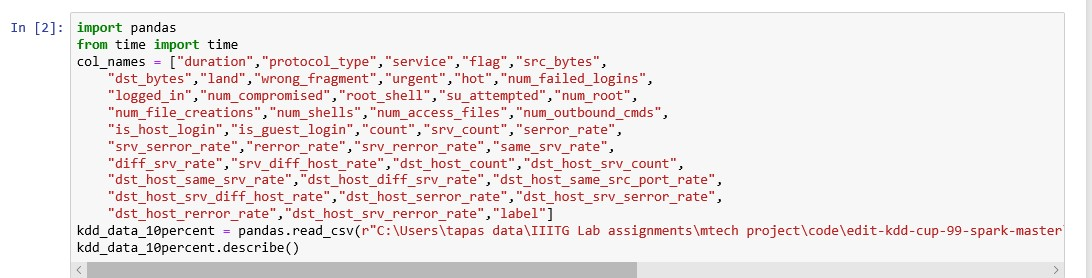
\includegraphics[width=15cm]{texfiles/images/code1.jpg}
    \caption{Initializing the dataset to feed in algorithm}
    \label{fig:code1}
\end{figure}
Some random thing Some random thing Some random thing Some random thing Some random thing Some random thing Some random thing Some random thing Some random thing Some random thing Some random thing Some random thing Some random thing Some random thing Some random thing Some random thing Some random thing Some random thing Some random thing Some random thing Some random thing Some random thing Some random thing  
\begin{figure}[H]
    \centering
    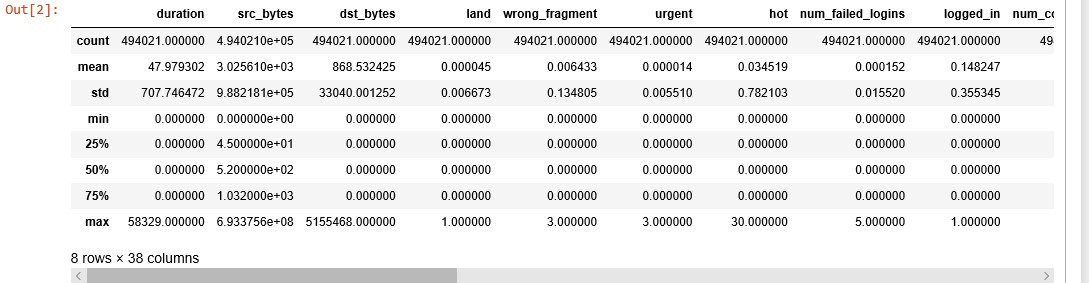
\includegraphics[width=15cm]{texfiles/images/code2.jpg}
    \caption{Output table generated after reading data}
    \label{fig:code2}
\end{figure}

Now we have our data loaded into a ``Pandas`` data frame. In order to get familiar with our data, let's have a look at how the labels are distributed. 
kdd\_data\_10percent['label'].value\_counts()
We get following attack types by reading the known attacks from the given dataset.
\begin{figure}[h]
    \centering
    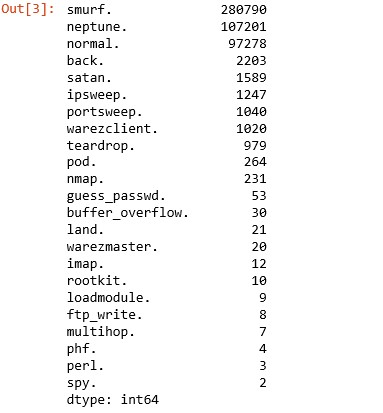
\includegraphics[height=7cm]{texfiles/images/code3.jpg}
    \caption{Attack types}
    \label{fig:code3}
\end{figure}
\subsection{Feature selection}

Some random thing Some random thing Some random thing Some random thing Some random thing Some random thing Some random thing Some random thing Some random thing Some random thing Some random thing Some random thing Some random thing Some random thing Some random thing Some random thing Some random thing Some random thing Some random thing Some random thing Some random thing Some random thing Some random thing  

Sklearn is a tool that helps dividing up the data into a test and a training set.
\begin{verbatim}
	from sklearn.model_selection import train_test_split
	
	features_train, features_test, labels_train, labels_test = train_test_split(
	features, labels, 
	test_size=0.20, random_state=42)
	
\end{verbatim}

Once the data is separated into test and training sets, we can begin to choose a classifier. 

\begin{verbatim}

	# import
from sklearn.neighbors import KNeighborsClassifier	

\end{verbatim}
KNearestneighbor can use any of the following 
algorithms ``auto``, ``ball\_tree``, ``kd\_tree``, ``brute``,the  default is ``auto``.
We can use any different classifier here other than RandomForestClassifier
sklearn is a toolkit which has various algorithms implemented and any of them can be choosen to 
implement a classifier depending upon what you want to do following shows implementation of RandomForestClassifier.

\begin{verbatim}
	# initialize
	clf = RandomForestClassifier()
	
	# train the classifier using the training data
	clf.fit(features_train, labels_train)
	
	# compute accuracy using test data
	acc_test = clf.score(features_test, labels_test)
	
	print ("Test Accuracy:", acc_test)
	
\end{verbatim}
A Some random thing Some random thing Some random thing Some random thing Some random thing Some random thing Some random thing Some random thing Some random thing Some random thing Some random thing Some random thing Some random thing Some random thing Some random thing Some random thing Some random thing Some random thing Some random thing Some random thing Some random thing Some random thing Some random thing  :
\begin{align}
	Precision &= \frac{True Positive}{True Positive+False Positive} \\
	Recall &= \frac{True Positive}{True Positive + False Negative} \\
	Accuracy(F1 score) &= 2 \times\frac{Precesion\times Recall}{Precision+Recall}
\end{align}

Some random thing Some random thing Some random thing Some random thing Some random thing Some random thing Some random thing Some random thing Some random thing Some random thing Some random thing Some random thing Some random thing Some random thing Some random thing Some random thing Some random thing Some random thing Some random thing Some random thing Some random thing Some random thing Some random thing  
\begin{verbatim}
from sklearn.metrics import recall_score, precision_score

precision = precision_score(labels_test, pred, average="weighted")
recall = recall_score(labels_test, pred, average="weighted")

print ("Precision:", precision) # 
print ("Recall:", recall) # 

\end{verbatim}

%\begin{figure}
%	\centering
%	\includegraphics{texfiles/images/}
%\end{figure}

Some random thing Some random thing Some random thing Some random thing Some random thing Some random thing Some random thing Some random thing Some random thing Some random thing Some random thing Some random thing Some random thing Some random thing Some random thing Some random thing Some random thing Some random thing Some random thing Some random thing Some random thing Some random thing Some random thing  
\begin{verbatim}
	from sklearn.svm import SVC
	clf = SVC
\end{verbatim}
Some random thing Some random thing Some random thing Some random thing Some random thing Some random thing Some random thing Some random thing Some random thing Some random thing Some random thing Some random thing Some random thing Some random thing Some random thing Some random thing Some random thing Some random thing Some random thing Some random thing Some random thing Some random thing Some random thing    
\begin{itemize}
	\item DOS: denial-of-service, e.g. syn flood;  
	\item R2L: unauthorized access from a remote machine, e.g. guessing password;  
	\item U2R:  unauthorized access to local superuser (root) privileges, e.g., various ``buffer overflow'' attacks;  
	\item probing: surveillance and other probing, e.g., port scanning.
\end{itemize}

 
 
  
